\subsection{Probabilistic Circuits và phân rã tensor}
\makeatletter
\@ifundefined{example}{\newtheorem{example}{Ví dụ}[subsection]}{}
\makeatother

\subsubsection{Giới thiệu và động lực}

Một phân phối xác suất đồng thời trên $N$ biến rời rạc $X_1, \ldots, X_N$ có thể
được nhìn nhận như một \emph{tensor xác suất}: mỗi phép gán
$\mathbf{x} = (x_1, \ldots, x_N)$ tương ứng với một phần tử
$p(\mathbf{x}) \geq 0$.  Kích thước của tensor này là
\begin{equation}
    |\mathcal{X}| = \prod_{n=1}^{N} |\mathcal{D}_n|,
\end{equation}
tăng theo hàm mũ khi $N$ lớn, nên việc dựng tường minh toàn bộ bảng xác suất
thường không khả thi. Hai hướng tiếp cận bổ sung nhau để vượt qua rào cản này là
tensor factorizations (xấp xỉ tensor bằng các nhân tử tensor có bậc thấp hơn) và circuits
(tổ chức phép tính dưới dạng computational graph để trả lời truy vấn mà không cần
dựng toàn bộ tensor) \cite{chrysos2025foundationsTutorial}.

Hai hướng này không hề độc lập với nhau. Mỗi tensor factorization có thể được mã hóa
chính xác như một circuit, và một deep circuit tương ứng với một hierarchical tensor
factorization \cite{chrysos2025foundationsTutorial, loconte2025relationship}.  Mối
liên hệ này quan trọng theo hai chiều:

\begin{itemize}[leftmargin=2em]
    \item Chiều TF $\to$ circuit: biết cách một tensor factorization hoạt động,
    ta biết cách xây một circuit tính đúng từng phần tử của nó.
    \item Chiều circuit $\to$ TF: các tính chất cấu trúc (structural properties)
    của circuit (smoothness, decomposability) tương ứng chính xác với điều kiện để
    một phân rã tensor hỗ trợ suy luận hiệu quả.
\end{itemize}

\begin{equation}
    \underbrace{\text{tensor factorizations}}_{\text{biểu diễn gọn}}
    \;\Longleftrightarrow\;
    \underbrace{\text{circuits}}_{\text{tổ chức phép tính}}
    \;\Longrightarrow\;
    \underbrace{\text{tractable inference}}_{\text{suy luận hiệu quả}}.
\end{equation}

Phần này trình bày bốn mục tiêu xây dựng dựa trên mối liên hệ đó
\cite{chrysos2025foundationsTutorial}: (1) thống nhất các tensor factorizations theo
cách module hóa (``Lego block approach''), (2) xây các factorization mới bằng cách
ghép layers, (3) thiết kế thuật toán tractable có hệ thống dựa trên structural
properties, và (4) coi tensor factorizations như generative models để lấy mẫu.

% ──────────────────────────────────────────────────────────────────────────────
\subsubsection{Circuit là gì?}

Xét tập biến $\mathbf{X}=\{X_1,\ldots,X_N\}$, trong đó mỗi biến
$X_i$ có miền giá trị $\mathcal{D}_i$.  Một phép gán đầy đủ được ký hiệu
$\mathbf{x}=(x_1,\ldots,x_N)$.  Với một tập con biến $S\subseteq\mathbf{X}$, ký
hiệu $\mathbf{x}_S$ là phần của phép gán $\mathbf{x}$ chỉ chứa các biến trong $S$.

\begin{definition}[Scope \cite{loconte2025relationship, chrysos2025foundationsTutorial}]
\label{def:circuit-scope}
\emph{Scope} của một unit $n$, ký hiệu $\mathrm{scope}(n)$, là tập biến mà hàm tại
unit đó phụ thuộc vào.  Nếu $\mathrm{scope}(n)=S$, output của unit $n$ được viết là
$c_n(\mathbf{x}_S)$.
\end{definition}

\begin{definition}[Circuit \cite{loconte2025relationship, chrysos2025foundationsTutorial}]
\label{def:circuit}
Một \emph{circuit} $c$ là một đồ thị có hướng không chu trình (DAG) tham số hóa.
Mỗi đỉnh là một computational unit, mỗi cạnh biểu diễn quan hệ phụ thuộc tính toán,
và $\mathrm{in}(n)$ là tập các unit đầu vào trực tiếp của unit $n$.  Circuit gồm
các input units, product units và sum units.  Nếu $o$ là output unit, giá trị của
circuit là
$c(\mathbf{x})=c_o(\mathbf{x}_{\mathrm{scope}(o)})$, được tính bằng một lượt
feedforward theo thứ tự topo.  Kích thước circuit, ký hiệu $|c|$, thường được tính
bằng số cạnh giữa các computational units.
\end{definition}

\begin{definition}[Các loại unit trong circuit \cite{loconte2025relationship}]
\label{def:circuit-units}
Các unit trong Definition~\ref{def:circuit} được định nghĩa đệ quy như sau:
\begin{enumerate}[label=(\roman*), leftmargin=2em]
    \item \textbf{Input unit}: nếu $n$ là unit lá với scope
    $S_n\subseteq\mathbf{X}$ và hàm cơ sở $f_n$, thì
    \begin{equation}
        \mathrm{scope}(n)=S_n,\qquad
        c_n(\mathbf{x}_{S_n}) = f_n(\mathbf{x}_{S_n}).
        \label{eq:circuit-input-unit}
    \end{equation}

    \item \textbf{Product unit}: nếu $n$ là product unit, thì
    \begin{equation}
        \mathrm{scope}(n)
        =
        \bigcup_{j \in \mathrm{in}(n)} \mathrm{scope}(j),
        \qquad
        c_n(\mathbf{x}_{\mathrm{scope}(n)})
        =
        \prod_{j \in \mathrm{in}(n)}
        c_j(\mathbf{x}_{\mathrm{scope}(j)}).
        \label{eq:circuit-product-unit}
    \end{equation}

    \item \textbf{Sum unit}: nếu $n$ là sum unit với trọng số $w_{n,j}\in\mathbb{R}$,
    thì
    \begin{equation}
        \mathrm{scope}(n)
        =
        \bigcup_{j \in \mathrm{in}(n)} \mathrm{scope}(j),
        \qquad
        c_n(\mathbf{x}_{\mathrm{scope}(n)})
        =
        \sum_{j \in \mathrm{in}(n)}
        w_{n,j}\,
        c_j(\mathbf{x}_{\mathrm{scope}(j)}).
        \label{eq:circuit-sum-unit}
    \end{equation}
\end{enumerate}
\end{definition}
% ──────────────────────────────────────────────────────────────────────────────
\subsubsection{Từ Tensor Factorization đến Circuit}

\paragraph{Cơ chế chuyển đổi.}
Với quan sát sau
\cite{chrysos2025foundationsTutorial}: \emph{một circuit có thể tính một tensor
entry tại một index bất kỳ}.  Với tensor $\mathcal{T}$ và một phép gán
$\mathbf{x} = (x_1, \ldots, x_N)$, bất kỳ công thức nào tính phần tử
$\mathcal{T}_{x_1 \cdots x_N}$ đều có thể được biểu diễn như một circuit $c$ sao
cho:
\begin{equation}
    \mathcal{T}_{x_1, \ldots, x_N} \approx c(x_1, \ldots, x_N).
\end{equation}

Đây là hướng chuyển TF $\to$ circuit.  Hướng ngược lại (circuit $\to$ TF) cũng
đúng: mỗi smooth và decomposable circuit mã hóa một multilinear polynomial, và
polynomial này tương ứng với một tensor factorization \cite{loconte2025relationship}.

\paragraph{CP decomposition như circuit.}
CP decomposition rank-$R$ của tensor bậc $N$ là:
\begin{equation}
    \mathcal{T}_{x_1, \ldots, x_N}
    \;\approx\;
    \sum_{r=1}^{R} \prod_{n=1}^{N} V^{(n)}_{x_n,\, r},
    \qquad \mathbf{V}^{(n)} \in \mathbb{R}^{I_n \times R}.
    \label{eq:cp-decomp}
\end{equation}
Phân tích cấu trúc của \eqref{eq:cp-decomp} theo góc nhìn circuit:
\begin{itemize}[leftmargin=2em]
    \item \textbf{Input layer}: với mỗi biến $X_n$ và giá trị $x_n$, layer trả về
    hàng $x_n$ của factor matrix $\mathbf{V}^{(n)}$, tức là vector
    $\bigl(V^{(n)}_{x_n,1}, \ldots, V^{(n)}_{x_n,R}\bigr)$.
    \item \textbf{Product layer}: nhân theo chiều rank, tính
    $\prod_{n=1}^{N} V^{(n)}_{x_n,r}$ cho mỗi $r$.
    \item \textbf{Sum layer}: cộng tổng trên $r = 1, \ldots, R$, cho ra
    $\sum_r (\cdots)$.
\end{itemize}
Cấu trúc ba tầng này là một CP layer \cite{chrysos2025foundationsTutorial}.

\begin{example}[Tính $c(1,2,2)$ theo CP decomposition bậc-3]
\label{ex:cp-eval}
Cho $R = 2$ và các factor matrices:
\[
\mathbf{V}^{(1)} = \begin{pmatrix} 0.1 & 1.2\\ 3.5 & -0.2\\ -0.1 & 0.2 \end{pmatrix},\quad
\mathbf{V}^{(2)} = \begin{pmatrix} 2.5 & 0.0\\ -3.4 & -0.5\\ -0.1 & 2.2 \end{pmatrix},\quad
\mathbf{V}^{(3)} = \begin{pmatrix} -2.3 & 1.0\\ 0.8 & -2.4\\ 0.7 & 1.5 \end{pmatrix}.
\]
Tại $x_1 = 1,\, x_2 = 2,\, x_3 = 2$ (chỉ số từ 0), circuit đọc từ factor matrices:
\begin{align*}
    \text{Input layer: } &
    (3.5,\,-0.2),\quad (-3.4,\,-0.5),\quad (0.8,\,-2.4). \\
    \text{Product: } &
    r=1:\; (3.5)(-3.4)(0.8) = -9.52, \quad
    r=2:\; (-0.2)(-0.5)(-2.4) = -0.24. \\
    \text{Sum: } &
    c(1,2,2) = -9.52 + (-0.24) = -9.76.
\end{align*}
Đây chính xác là ví dụ được trình bày trong tutorial \cite{chrysos2025foundationsTutorial}.
\end{example}

\paragraph{Tucker decomposition như circuit.}
Tucker decomposition tổng quát hóa CP bằng cách đưa vào một core tensor
$\mathcal{W} \in \mathbb{R}^{R_1 \times \cdots \times R_N}$ kiểm soát cách trộn
các latent components:
\begin{equation}
    \mathcal{T}_{x_1, \ldots, x_N}
    \;\approx\;
    \sum_{r_1=1}^{R_1} \cdots \sum_{r_N=1}^{R_N}
    \mathcal{W}_{r_1, \ldots, r_N}
    \prod_{n=1}^{N} V^{(n)}_{x_n,\, r_n}.
    \label{eq:tucker-decomp}
\end{equation}
Với circuit, factor matrices cung cấp input layers (tương tự CP),
product layer kết hợp các mode, còn sum layer cộng trên tất cả bộ chỉ số
$(r_1, \ldots, r_N)$ với trọng số lấy từ các phần tử của $\mathcal{W}$.  Khi
$\mathcal{W}$ là diagonal với $R_1 = \cdots = R_N = R$, Tucker suy biến thành CP.
Mệnh đề tổng quát hóa điều này:

\begin{proposition}[Tucker như circuit, phát biểu trong \cite{loconte2025relationship}]
\label{prop:tucker-circuit}
Cho $\mathcal{T} \in \mathbb{R}^{I_1 \times \cdots \times I_N}$ và Tucker
factorization multilinear rank $(R_1, \ldots, R_N)$ như trong~\eqref{eq:tucker-decomp}.
Tồn tại một circuit $c$ trên các biến $X_1, \ldots, X_N$ với $\mathrm{dom}(X_n) =
[I_n]$ tính cùng factorization, và kích thước circuit thỏa
$|c| \in \mathcal{O}\!\left(N \prod_{n=1}^{N} R_n\right)$.
\end{proposition}

\paragraph{Định nghĩa tensor hóa của circuit.}
Circuit với ba quy tắc tổ hợp, cho phép ta xây dựng circuit từng
tầng một \cite{chrysos2025foundationsTutorial}:
\begin{enumerate}[label=\Roman*.]
    \item Một tập các hàm tractable là một circuit layer.
    \item Một linear projection của một layer là một circuit layer:
    $\mathbf{c}(\mathbf{x}) = \mathbf{W}\boldsymbol{\ell}(\mathbf{x})$,
    $\mathbf{W} \in \mathbb{R}^{K \times M}$.
    \item Tích của hai layers là một circuit layer---Hadamard:
    $\mathbf{c}(\mathbf{x}) = \boldsymbol{\ell}(\mathbf{x}) \ast \mathbf{r}(\mathbf{x})$,
    hoặc Kronecker:
    $\mathbf{c}(\mathbf{x}) = \operatorname{vec}\!\left(\boldsymbol{\ell}(\mathbf{x})\mathbf{r}(\mathbf{x})^{\top}\right)$.
\end{enumerate}
Xếp chồng nhiều layers theo ba quy tắc này cho ra một \emph{deep circuit}.

\paragraph{Lego block approach.}
Mỗi loại factorization tương ứng với một ``block'', và ta tạo factorization mới bằng cách
ghép các blocks lại \cite{chrysos2025foundationsTutorial}:
\begin{itemize}[leftmargin=2em]
    \item \textbf{CP layer}: tích Hadamard của các input vectors, sau đó cộng---tương
    đương CP.
    \item \textbf{Tucker layer}: tích Kronecker của các input vectors, sau đó nhân
    với ma trận trọng số $\mathbf{W}$---tương đương Tucker.
    \item \textbf{Monarch layer}: sử dụng Monarch matrix factorization
    $\mathbf{W}_M = \mathbf{P}_L \mathbf{L} \mathbf{P}_R \mathbf{R}$ để làm
    weight matrix, mở rộng pipeline với các factorization có cấu trúc
    \cite{chrysos2025foundationsTutorial}.
\end{itemize}
Bằng cách stack các blocks khác nhau, ta thu được hierarchical factorizations sâu hơn
và có thể chia sẻ sub-factorizations giữa các nhánh của circuit để tiết kiệm tính toán
\cite{loconte2025relationship}.

\paragraph{Ý nghĩa của việc deep hơn.}
Một lợi thế quan trọng của deep circuits là hiệu quả biểu diễn: đôi khi circuit sâu
có thể biểu diễn cùng một hàm với số tham số ít hơn theo hàm mũ so với circuit nông
\cite{loconte2025relationship}. Điều này phản ánh ưu điểm tương tự của hierarchical
Tucker so với shallow Tucker: nó cần số rank nhỏ hơn đáng kể để đạt cùng mức xấp xỉ.

% ──────────────────────────────────────────────────────────────────────────────
\subsubsection{Từ Circuit đến Tractable Inference qua Structural Properties}

Sau khi mã hóa tensor factorization thành circuit, câu hỏi đặt ra là: circuit đó
có thể trả lời những truy vấn nào một cách hiệu quả?  Câu trả lời phụ thuộc vào
\emph{structural properties} của circuit \cite{vergari2021compositional}.

\begin{definition}[Smoothness \cite{vergari2021compositional}]
\label{def:smoothness}
Circuit là \emph{smooth} nếu mọi sum unit chỉ cộng các input units có cùng scope:
\begin{equation}
    \forall n \in \mathcal{S},\;
    \forall i, j \in \mathrm{in}(n):\quad
    \mathrm{scope}(i) = \mathrm{scope}(j).
\end{equation}
\end{definition}

\begin{definition}[Decomposability \cite{vergari2021compositional}]
\label{def:decomposability}
Circuit là \emph{decomposable} nếu mọi product unit chỉ nhân các input units có
scope rời nhau từng đôi một:
\begin{equation}
    \forall n \in \mathcal{P},\;
    \forall i \neq j \in \mathrm{in}(n):\quad
    \mathrm{scope}(i) \cap \mathrm{scope}(j) = \varnothing.
\end{equation}
\end{definition}

Tại sao hai tính chất này lại quan trọng?  Nhờ decomposability, tích phân trên
product node tách thành tích của các tích phân độc lập trên các nhóm biến rời nhau:
\begin{equation}
    \int p_A(\mathbf{x}_A)\, p_B(\mathbf{x}_B)\;
    d\mathbf{x}_A\, d\mathbf{x}_B
    = \left(\int p_A(\mathbf{x}_A)\, d\mathbf{x}_A\right)
      \left(\int p_B(\mathbf{x}_B)\, d\mathbf{x}_B\right),
    \quad A \cap B = \varnothing.
    \label{eq:factored-integral}
\end{equation}
Kết hợp smoothness và decomposability, mọi marginal và conditional đều có thể tính
trong một feedforward pass duy nhất qua circuit
\cite{chrysos2025foundationsTutorial, vergari2021compositional}. Đây cũng là hệ
quả của \emph{multilinearity}:
\begin{equation}
    \text{Smoothness} \wedge \text{Decomposability}
    \;\Rightarrow\;
    \text{Multilinearity của circuit}.
\end{equation}

\begin{definition}[Compatibility \cite{vergari2021compositional}]
\label{def:compatibility}
Hai circuits là \emph{compatible} nếu chúng phân rã scope theo cùng một cấu trúc.
Điều kiện đủ phổ biến: hai deep circuits chia sẻ cùng tree region graph, tức là mỗi
cặp product units có cùng scope ở hai circuits đều chia scope đó thành cùng child
scopes.
\end{definition}

\begin{definition}[Determinism \cite{vergari2021compositional}]
\label{def:determinism}
Circuit là \emph{deterministic} nếu các input của mọi sum unit được định nghĩa trên
các supports rời nhau:
\begin{equation}
    \forall n \in \mathcal{S},\;
    \forall i \neq j \in \mathrm{in}(n):\quad
    \mathrm{supp}(c_i) \cap \mathrm{supp}(c_j) = \varnothing.
\end{equation}
\end{definition}

Liên kết trực tiếp với tensor factorizations: Tucker factorization khi biểu diễn
như circuit (Proposition~\ref{prop:tucker-circuit}) \emph{tự động} là smooth và
decomposable, do factor matrices của các mode khác nhau có scope rời nhau
\cite{loconte2025relationship}.  Điều này có nghĩa là bất kỳ Tucker factorization
nào cũng tự nhiên hỗ trợ marginal inference hiệu quả khi nhìn qua lăng kính circuit.

Bảng~\ref{tab:properties} tóm tắt các tổ hợp structural properties và lớp truy vấn
tractable tương ứng:

\begin{table}[h]
\centering
\caption{Structural properties và các query classes tractable
         \cite{chrysos2025foundationsTutorial, vergari2021compositional}.}
\label{tab:properties}
\begin{tabular}{@{}lll@{}}
\toprule
\textbf{Properties} & \textbf{Query class} & \textbf{Cơ chế} \\
\midrule
Smoothness + Decomposability & Marginals / integrals tùy ý & Một feedforward pass \\
Smoothness + Compatibility   & Expectation $\mathbb{E}_{\mathbf{x} \sim p}[f(\mathbf{x})]$ & Tích hai circuits \\
Decomposability              & Partition function, conditionals & Tuyến tính theo $|c|$ \\
Determinism + Decomposability & MAP inference & Tối ưu tractable \\
\bottomrule
\end{tabular}
\end{table}

% ──────────────────────────────────────────────────────────────────────────────
\subsubsection{Probabilistic Circuits: Non-negative Tensor Factorizations như Mô hình Xác suất}

Bước tiếp theo là thêm ràng buộc \emph{không âm} để circuit mã hóa một phân phối
xác suất hợp lệ.  Đây là nơi non-negative tensor factorization gặp probabilistic
circuits.

\begin{definition}[Probabilistic Circuit \cite{choi2021probabilistic, loconte2025relationship}]
\label{def:pc}
Một \emph{probabilistic circuit} (PC) là một circuit $c$ thỏa
$c(\mathbf{x}) \geq 0$ với mọi $\mathbf{x}$.  Phân phối xác suất thu được bằng
chuẩn hóa:
\begin{equation}
    p(\mathbf{x}) = \frac{c(\mathbf{x})}{Z},
    \qquad
    Z =
    \begin{cases}
        \displaystyle\sum_{\mathbf{x}} c(\mathbf{x}), & \text{rời rạc},\\[4pt]
        \displaystyle\int c(\mathbf{x})\, d\mathbf{x}, & \text{liên tục}.
    \end{cases}
    \label{eq:pc-normalize}
\end{equation}
Một điều kiện đủ thường dùng là ràng buộc các tham số của sum units và đầu ra của
input units không âm; khi đó circuit là một \emph{monotonic PC}
\cite{loconte2025relationship}.
\end{definition}

Liên hệ với tensor factorizations: một \emph{non-negative Tucker factorization}
(tất cả phần tử của $\mathcal{W}$ và $\mathbf{V}^{(n)}$ đều không âm) chính là
một PC monotonic.  Nói cách khác, bất kỳ non-negative Tucker (hay CP, HOSVD) nào
cũng là một PC với tất cả các ưu điểm về tractable inference \cite{loconte2025relationship}.

Input functions không nhất thiết chỉ là embedding entries $f(x) = v_{x,r}$.  Chúng
có thể được thay bằng \textbf{PMF} (Binomial, Categorical),
continuous distributions ($\mathcal{N}(\mu,\sigma^2)$, splines, polynomials), hoặc
thậm chí các deep generative models \cite{loconte2025relationship}. Khi input functions là hàm liên tục, tensor
tương ứng trở thành \emph{infinite-dimensional} và circuit mã hóa một \textbf{PDF} thay vì \textbf{PMF}.

\begin{example}[Non-negative CP factorization là PC]
\label{ex:nn-cp-pc}
Xét CP factorization rank-$R$ trên hai biến rời rạc $(X_1, X_2)$ với
$\mathbf{V}^{(1)}, \mathbf{V}^{(2)} \geq 0$ (tất cả phần tử không âm):
\begin{equation}
    c(x_1, x_2) = \sum_{r=1}^{R} V^{(1)}_{x_1, r}\, V^{(2)}_{x_2, r} \geq 0.
\end{equation}
Circuit tương ứng có $2R$ input nodes, $R$ product nodes và 1 sum node.  Nó smooth
(sum node: tất cả input có scope $\{X_1, X_2\}$), decomposable (mỗi product node
có input từ $\{X_1\}$ và $\{X_2\}$ riêng biệt), và không âm---do đó là PC.
Phân phối sau chuẩn hóa là:
$p(x_1, x_2) = c(x_1, x_2) / Z$, $Z = \sum_{x_1, x_2} c(x_1, x_2)$.
\end{example}

\begin{figure}[h]
\centering
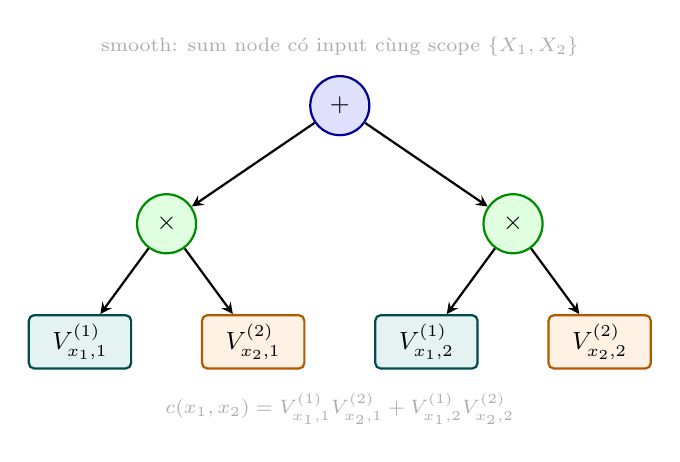
\begin{tikzpicture}[
    every node/.style={font=\small},
    op/.style={circle, draw, thick, minimum size=0.75cm, align=center},
    leaf/.style={draw, rounded corners=2pt, thick, minimum width=1.3cm,
                 minimum height=0.65cm, align=center},
    edge/.style={->, >=stealth, thick},
    ann/.style={font=\scriptsize, text=gray!65}
]
    % sum node
    \node[op, fill=blue!12, draw=blue!60!black] (s0) at (0, 3.0) {$+$};
    % product nodes
    \node[op, fill=green!12, draw=green!55!black] (p1) at (-2.2, 1.5) {$\times$};
    \node[op, fill=green!12, draw=green!55!black] (p2) at ( 2.2, 1.5) {$\times$};
    % input nodes
    \node[leaf, fill=teal!10,   draw=teal!60!black]   (v11) at (-3.3, 0) {$V^{(1)}_{x_1,1}$};
    \node[leaf, fill=orange!10, draw=orange!70!black]  (v21) at (-1.1, 0) {$V^{(2)}_{x_2,1}$};
    \node[leaf, fill=teal!10,   draw=teal!60!black]   (v12) at ( 1.1, 0) {$V^{(1)}_{x_1,2}$};
    \node[leaf, fill=orange!10, draw=orange!70!black]  (v22) at ( 3.3, 0) {$V^{(2)}_{x_2,2}$};
    % edges
    \draw[edge] (s0) -- (p1);
    \draw[edge] (s0) -- (p2);
    \draw[edge] (p1) -- (v11);
    \draw[edge] (p1) -- (v21);
    \draw[edge] (p2) -- (v12);
    \draw[edge] (p2) -- (v22);
    % annotations
    \node[ann, align=center] at (0, 3.75)
        {smooth: sum node có input cùng scope $\{X_1, X_2\}$};
    \node[ann, align=center] at (0,-0.85)
        {$c(x_1,x_2) = V^{(1)}_{x_1,1}V^{(2)}_{x_2,1}
         + V^{(1)}_{x_1,2}V^{(2)}_{x_2,2}$};
\end{tikzpicture}
\caption{Non-negative CP factorization rank-2 trên $(X_1,X_2)$ biểu diễn như
circuit. Input layers đọc hàng tương ứng từ factor matrices; product nodes
thực hiện tích theo mode; sum node cộng tổng trên rank. Circuit tự động smooth
và decomposable, do đó là PC hỗ trợ marginal inference hiệu quả.}
\label{fig:cp-as-pc}
\end{figure}

% ──────────────────────────────────────────────────────────────────────────────
\subsubsection{Suy luận hiệu quả và diễn giải Latent Variable}

\paragraph{Marginal inference.}
Cho tập biến ẩn $X_M \subseteq X$ và biến quan sát $X_O = X \setminus X_M$,
marginal là:
\begin{equation}
    p(\mathbf{x}_O) = \sum_{\mathbf{x}_M \in \mathcal{D}_M}
                     p(\mathbf{x}_O,\, \mathbf{x}_M).
    \label{eq:marginal}
\end{equation}
Với PC smooth và decomposable, tổng này tính được trong một feedforward pass duy
nhất qua circuit, tuyến tính theo kích thước circuit
\cite{loconte2025relationship, vergari2021compositional}.

Nhìn dưới góc độ tensor factorization, marginal inference chính là phép \emph{sum-out}
trên các mode tương ứng với $X_M$.  Nếu PC mã hóa một CP factorization không âm:
\begin{equation}
    c(x_1,\ldots,x_N)
    =
    \sum_{r=1}^{R}\prod_{n=1}^{N}V^{(n)}_{x_n,r},
    \qquad V^{(n)}_{x_n,r}\ge 0,
    \label{eq:nn-cp-query}
\end{equation}
thì việc marginalize các biến trong $M$ không cần dựng tensor đầy đủ.  Ta chỉ cần
thay mỗi factor của một mode bị loại bằng tổng theo hàng của mode đó:
\begin{equation}
    c(\mathbf{x}_O)
    =
    \sum_{r=1}^{R}
    \left(\prod_{n\in O}V^{(n)}_{x_n,r}\right)
    \left(\prod_{m\in M}\sum_{x_m\in\mathcal{D}_m}V^{(m)}_{x_m,r}\right).
    \label{eq:cp-marginal-query}
\end{equation}
Vì mỗi product node trong CP gom các factor có scope rời nhau, phép tổng trên nhiều
assignment được đẩy xuống từng factor matrix.  Đây là ý nghĩa TF của điều kiện
decomposability: một phép cộng có vẻ theo cấp số mũ được biến thành các phép tổng nhỏ
trên từng mode.

\paragraph{Expectation và reasoning về ML models.}
Khi cả $p(\mathbf{x})$ lẫn $f(\mathbf{x})$ đều là circuits compatible:
\begin{equation}
    \mathbb{E}_{\mathbf{x} \sim p}[f(\mathbf{x})]
    = \int p(\mathbf{x})\, f(\mathbf{x})\, d\mathbf{x},
    \label{eq:expectation}
\end{equation}
có thể tính trong thời gian $\mathcal{O}(|p| \cdot |f|)$.
Ở đây không cần chuyển hai circuit sang TF để tính: bản thân phép product giữa hai
compatible circuits rồi marginalize đã cho thuật toán tractable.  Vai trò của TF là
diễn giải cùng phép tính đó dưới dạng đại số tensor.  Trong ngôn ngữ TF, đây là inner
product giữa tensor xác suất của $p$ và tensor hàm
của $f$:
\begin{equation}
    \langle \mathcal{P}, \mathcal{F}\rangle
    =
    \sum_{\mathbf{x}}\mathcal{P}_{\mathbf{x}}\mathcal{F}_{\mathbf{x}}.
\end{equation}
Nếu $\mathcal{P}$ và $\mathcal{F}$ được biểu diễn bởi hai factorization có cùng cách
phân rã scope, ta có thể contract trực tiếp các factor tương ứng thay vì materialize hai
tensor đầy đủ.  Điều kiện compatibility trong circuit chính là điều kiện để hai TF
``khớp cấu trúc'' khi nhân và lấy tổng \cite{loconte2025relationship,
vergari2021compositional}.

Tutorial đặt ra ba câu hỏi thực tế dạng expectation này
\cite{chrysos2025foundationsTutorial}:
\begin{align}
    \text{Missing values:}\quad &
    \int p(\mathbf{x}_O,\, \mathbf{x}_M)\, d\mathbf{x}_M,\\
    \text{Fairness:}\quad &
    \mathbb{E}[f(\mathbf{x}) \mid a=0] - \mathbb{E}[f(\mathbf{x}) \mid a=1],\\
    \text{Adversarial robustness:}\quad &
    \mathbb{E}_{\boldsymbol{\varepsilon} \sim p_{\mathrm{noise}}}
    [f(\mathbf{x} + \boldsymbol{\varepsilon})].
\end{align}

\paragraph{Missing values dưới dạng TF.}
Missing-value query là marginal hoặc conditional query.  Các mode quan sát $O$ được
giữ cố định tại $\mathbf{x}_O$, còn các mode missing $M$ được sum-out để tính mẫu số:
\begin{equation}
    p(\mathbf{x}_M\mid \mathbf{x}_O)
    =
    \frac{p(\mathbf{x}_O,\mathbf{x}_M)}
         {\sum_{\mathbf{x}'_M}p(\mathbf{x}_O,\mathbf{x}'_M)}.
    \label{eq:missing-conditional}
\end{equation}
Với CP trong~\eqref{eq:nn-cp-query}, tử số chỉ là đánh giá factorization tại
$(\mathbf{x}_O,\mathbf{x}_M)$; mẫu số dùng đúng phép sum-out trong
\eqref{eq:cp-marginal-query}.  Do đó TF biểu diễn missing-value inference bằng hai
thao tác: \emph{fix mode} cho biến quan sát và \emph{contract/sum mode} cho biến
missing.

\paragraph{Fairness dưới dạng TF.}
Query fairness trong tutorial so sánh hai kỳ vọng có điều kiện theo biến nhạy cảm
$A$:
\begin{equation}
    \mathbb{E}[f(\mathbf{x})\mid A=0]
    -
    \mathbb{E}[f(\mathbf{x})\mid A=1].
\end{equation}
Dưới góc nhìn TF, điều kiện $A=a$ tương ứng với việc chọn slice của factorization tại
mode $A$.  Sau khi cố định slice đó, ta contract các mode còn lại với tensor/circuit
biểu diễn $f$.  Nếu $p$ và $f$ compatible, hai kỳ vọng có điều kiện vẫn được tính bằng
cùng một cơ chế: fix một mode, nhân hai factorization, rồi sum-out các mode còn lại.

\paragraph{Adversarial robustness dưới dạng TF.}
Với query
\begin{equation}
    \mathbb{E}_{\boldsymbol{\varepsilon}\sim p_{\mathrm{noise}}}
    [f(\mathbf{x}+\boldsymbol{\varepsilon})],
\end{equation}
tensor xác suất đến từ distribution của nhiễu, còn tensor hàm đến từ response
$f(\mathbf{x}+\boldsymbol{\varepsilon})$.  Nếu response này cũng được mã hóa bởi một
circuit/TF compatible với $p_{\mathrm{noise}}$, query vẫn là một phép contraction giữa
hai factorization.  Ngược lại, khi $f$ là neural network thông thường, tutorial nhấn
mạnh rằng compatibility không còn áp dụng; lúc đó sampling từ PC là cách xấp xỉ tự
nhiên \cite{chrysos2025foundationsTutorial}.

\begin{table}[h]
\centering
\caption{Cách nhìn tensor factorization của các query suy luận trong tutorial.}
\label{tab:tf-view-of-queries}
\begin{tabular}{@{}p{0.22\textwidth}p{0.34\textwidth}p{0.34\textwidth}@{}}
\toprule
\textbf{Query} & \textbf{Dạng toán học} & \textbf{Thao tác trên TF} \\
\midrule
Marginal &
$\sum_{\mathbf{x}_M}p(\mathbf{x}_O,\mathbf{x}_M)$ &
Sum-out/contract các mode trong $M$. \\
Missing values &
$p(\mathbf{x}_M\mid\mathbf{x}_O)$ &
Fix mode quan sát, sum-out mode missing để chuẩn hóa. \\
Expectation &
$\sum_{\mathbf{x}}p(\mathbf{x})f(\mathbf{x})$ &
Inner product/contraction giữa hai factorization compatible. \\
Fairness &
$\mathbb{E}[f\mid A=0]-\mathbb{E}[f\mid A=1]$ &
Chọn slice theo mode nhạy cảm rồi contract các mode còn lại. \\
Adversarial robustness &
$\mathbb{E}_{\varepsilon\sim p_{\mathrm{noise}}}[f(\mathbf{x}+\varepsilon)]$ &
Contract nếu response có TF compatible; nếu không thì sampling. \\
Sampling &
$p(\mathbf{x})=\sum_z p(z)p(\mathbf{x}\mid z)$ &
Diễn giải rank/sum index như latent variable và sinh mẫu backward. \\
\bottomrule
\end{tabular}
\end{table}

\paragraph{Non-negative factorizations như latent variable models.}
Non-negative tensor factorizations, khi được biểu diễn như monotonic PCs, không chỉ
hỗ trợ marginal inference mà còn có thể được đọc như các mô hình sinh với biến ẩn
rời rạc \cite{loconte2025relationship}.
Chìa khóa là diễn giải mỗi sum node như một mixture với biến latent $Z$:
\begin{equation}
    p(\mathbf{x}) = \sum_{z=1}^{K} p(z)\, p(\mathbf{x} \mid z),
    \qquad p(z) \geq 0,\quad \sum_z p(z) = 1.
    \label{eq:sum-mixture}
\end{equation}
Trong CP không âm, chỉ số rank $r$ trong~\eqref{eq:nn-cp-query} đóng vai trò một
latent component.  Nếu các factor được chuẩn hóa thành các phân phối hợp lệ và trọng
số trộn tổng bằng 1, ta có thể đọc CP như một mixture:
\begin{equation}
    p(\mathbf{x})
    =
    \sum_{r=1}^{R}p(r)\prod_{n=1}^{N}p_n(x_n\mid r).
    \label{eq:cp-latent-mixture}
\end{equation}
Như vậy, một component CP không chỉ là một pattern đồng thời trên các mode, mà còn là
một trạng thái latent sinh ra các biến quan sát theo từng mode.  Với Tucker hoặc deep
TF, các sum units tạo ra nhiều latent variables rời rạc theo cấu trúc phân cấp của
circuit; số latent variables tương ứng với số sum units trong PC
\cite{loconte2025relationship}.

Product node cho phép lấy mẫu độc lập trên các nhóm biến rời nhau
($A \cap B = \varnothing$):
\begin{equation}
    c(\mathbf{x}_A, \mathbf{x}_B) = c_A(\mathbf{x}_A)\, c_B(\mathbf{x}_B).
\end{equation}
Với smooth và decomposable PC đã chuẩn hóa, sampling có thể thực hiện bằng backward
traversal qua circuit: tại sum layer ta lấy mẫu biến ẩn categorical, tại product layer
ta tiếp tục xuống tất cả các nhánh có scope rời nhau, và tại input layer ta lấy mẫu
từ phân phối lá. Thuật toán này chạy tuyến tính theo kích thước circuit
\cite{loconte2025relationship, choi2021probabilistic}:
\begin{equation}
    \begin{array}{ll}
        \text{Sum node:}     & z \sim \mathrm{Categorical}(w_1,\ldots,w_K),
                               \text{ đi vào nhánh } z, \\[1mm]
        \text{Product node:} & \mathbf{x}_A \sim p_A,\;
                               \mathbf{x}_B \sim p_B \text{ độc lập}, \\[1mm]
        \text{Input node:}   & x_n \sim p_n(x_n),\;
                               \text{e.g. Categorical hoặc Gaussian.}
    \end{array}
    \label{eq:sampling}
\end{equation}
Đây là lý do tại sao non-negative tensor factorizations---khi nhìn như circuits---
không chỉ cung cấp xấp xỉ tensor, mà còn là \emph{generative models} với khả năng
lấy mẫu chính xác và hiệu quả \cite{loconte2025relationship}.

% ──────────────────────────────────────────────────────────────────────────────
\subsubsection{Ứng dụng, Liên hệ và Các Vấn đề Còn Mở}

\paragraph{Tractable models trong intractable pipelines.}
Chiến lược thực tế là dùng PC ở những điểm trong pipeline cần suy luận chính xác
(marginalization, expectation), trong khi phần còn lại có thể là neural networks
không tractable.  Ví dụ điển hình là tractable conditioning over every missing mask:
PC xử lý marginal inference, kết quả được truyền vào neural network encoder/decoder,
và cách tiếp cận này cho kết quả tốt hơn (V)AE trên bài toán imputation
\cite{braun2025tractable}.

\paragraph{Mở rộng: Từ Tensor rời rạc đến Hàm liên tục.}
Khi input functions là hàm liên tục (Gaussian, spline, polynomial), tensor xác suất
tương ứng trở thành \emph{infinite-dimensional}---một quasi-tensor theo thuật ngữ
của \cite{loconte2025relationship}.  Circuit lúc đó mã hóa một PDF thay vì PMF,
với công thức chuẩn hóa dùng tích phân thay vì tổng.  Quasi-tensors có thể được
biểu diễn bằng circuits trên các biến có miền vô hạn; việc thêm \emph{integral
units} cho phép xem một lớp PC gần đây như các factorization liên tục hoặc
infinite-rank \cite{loconte2025relationship}.  Đây là cơ sở đúng cho Probabilistic
Integral Circuits và các mô hình latent liên tục mở rộng từ PC
\cite{loconte2025relationship, gala2024probabilisticIntegral, gala2024scalingContinuous}.

\paragraph{Hạn chế: tractable không đồng nghĩa với biểu diễn luôn gọn.}
Các structural properties như smoothness và decomposability giúp suy luận chính xác
trở nên tractable, nhưng chúng không bảo đảm rằng mọi phân phối đều có một circuit
nhỏ.  Đây là điểm cần phân biệt rõ: \emph{tractability} nói về chi phí trả lời truy
vấn khi circuit đã được cho trước, còn \emph{expressiveness/compactness} nói về việc
cần circuit lớn đến mức nào để biểu diễn hoặc xấp xỉ một phân phối.

Với Tucker factorization, nếu tensor xác suất bậc $N$ được viết với multilinear rank
$(R_1,\ldots,R_N)$ thì riêng core tensor đã có
\begin{equation}
    \prod_{n=1}^{N} R_n
\end{equation}
tham số.  Khi $R_1=\cdots=R_N=R$, kích thước core là $R^N$, tức tăng theo hàm mũ theo
số biến/mode.  Vì vậy, nếu một phân phối cần rank lớn để biểu diễn tốt, shallow
Tucker hoặc CP không còn là biểu diễn gọn, dù circuit tương ứng vẫn hỗ trợ một số
truy vấn suy luận hiệu quả sau khi đã được xây dựng.  Nói cách khác, tồn tại những
phân phối có tương tác bậc cao hoặc phụ thuộc phức tạp khiến rank cần thiết tăng rất
nhanh; lúc đó việc học và lưu trữ mô hình có thể trở thành nút thắt chính
\cite{loconte2025relationship}.

Deep circuits/hierarchical factorizations giảm vấn đề này bằng cách chia nhỏ scope và
chia sẻ sub-factorizations, nhưng đây không phải bảo đảm phổ quát.  Hiệu quả biểu
diễn phụ thuộc mạnh vào region graph, loại layer, rank/width, và mức độ phù hợp giữa
cấu trúc circuit với phụ thuộc thật trong dữ liệu.  Nếu chọn cấu trúc sai, ta vẫn có
thể cần width rất lớn, thậm chí tăng theo hàm mũ, để đạt xấp xỉ tốt.

\paragraph{Các thách thức nghiên cứu còn mở.}
Tutorial kết thúc với bốn câu hỏi chưa được giải quyết
\cite{chrysos2025foundationsTutorial}:
\begin{enumerate}[label=\textbf{\arabic*.}, leftmargin=2em]
    \item \textbf{Optimization}: không chỉ là chọn một optimizer như SGD hay Adam,
    mà là hiểu bài toán học tham số và học cấu trúc của circuit/factorization.  Với
    shallow factorizations, ta có một số phân tích về hội tụ, local minima hoặc điều
    kiện khôi phục trong các thiết lập đơn giản.  Câu hỏi mở là liệu các kết quả này
    có thể mở rộng sang deep circuits, nơi loss vẫn không lồi nhưng còn phụ thuộc vào
    region graph, cách ghép layers, width/rank và các ràng buộc tractability hay
    không.
    \item \textbf{Identifiability}: khi nào deep circuit có biểu diễn duy nhất
    (khôi phục được ground truth)?
    \item \textbf{Approximate inference}: xây dựng property-driven approximate
    algorithms theo cách hệ thống như thế nào?
    \item \textbf{Scalability}: mở rộng ứng dụng circuits lên hàng triệu biến và
    constraints.
\end{enumerate}
